\documentclass[12pt,a4paper,onecolumn]{article}
\usepackage[utf8]{inputenc}
\usepackage[T1]{fontenc}
\usepackage[french]{babel}

\usepackage{multicol}
\usepackage{fullpage}

% ------------------------- Color table ----------------------------------------
\usepackage{multirow}
\usepackage[table]{xcolor}
\definecolor{maroon}{cmyk}{0,0.87,0.68,0.32}
\usepackage{booktabs} % to make prettier tables (toprule, midrule, bottomrule)
% ------------------------------------------------------------------------------

\usepackage{amscd}
\usepackage{amsthm}
\usepackage{physics}
\usepackage{fullpage}
\usepackage{textcomp,gensymb} %pour le °C, et textcomp pour éviter les warning
\usepackage{graphicx} %pour les images
\usepackage{caption}
\usepackage{subcaption}
\usepackage[colorlinks=true,
	breaklinks=true,
	citecolor=blue,
	linkcolor=blue,
	urlcolor=blue]{hyperref} % pour insérer des liens
\usepackage{epstopdf} %converting to PDF
\usepackage[export]{adjustbox} %for large figures

\usepackage{array}
\usepackage{dsfont}% indicatrice : \mathds{1}


% -------------------------- Mathematics ---------------------------------------
\graphicspath{{images/}{../images/}} % For the images path
% ------------------------------------------------------------------------------

% -------------------------- Mathematics ---------------------------------------
\usepackage{mathrsfs, amsmath, amsfonts, amssymb}
\usepackage{bm}
\usepackage{mathtools}
\usepackage[Symbol]{upgreek} % For pi \uppi different from /pi

% For pseudo-code
\usepackage[ruled,vlined,linesnumbered,noresetcount]{algorithm2e}

\newcommand{\R}{\mathbb{R}} % For Real space
\usepackage{tikz}
\usetikzlibrary{bayesnet} %library to draw graphical models1
% ------------------------------------------------------------------------------


% -------------------------- Code format ---------------------------------------
\usepackage[numbered,framed]{matlab-prettifier}
\lstset{
	style              = Matlab-editor,
	basicstyle         = \mlttfamily,
	escapechar         = '',
	mlshowsectionrules = true,
}
% ------------------------------------------------------------------------------

% ------------------------- Blbiographie --------------------------------------
\usepackage[backend=biber, style=ieee]{biblatex}
\addbibresource{biblio.bib}
\usepackage{csquotes}
% ------------------------------------------------------------------------------


\setcounter{tocdepth}{4} %Count paragraph
\setcounter{secnumdepth}{4} %Count paragraph
\usepackage{float}

\usepackage{graphicx} % for graphicspath
% \graphicspath{{../images/}}

\usepackage{array,tabularx}
\newcolumntype{L}[1]{>{\raggedright\let\newline\\\arraybackslash\hspace{0pt}}m{#1}}
\newcolumntype{C}[1]{>{\centering\let\newline\\\arraybackslash\hspace{0pt}}m{#1}}
\newcolumntype{R}[1]{>{\raggedleft\let\newline\\\arraybackslash\hspace{0pt}}m{#1}}


\usepackage{hyperref}

% \setcounter{section}{5} % to start counting section to 6

% Independent sign
\newcommand{\indep}{\ensuremath{\,\bot\!\!\!\bot\,}} %% The symbol for independent

% Alpha / Numbers for sections
\renewcommand{\thesubsubsection}{\arabic{section}.\arabic{subsection}.\alph{subsubsection})}

% Norm
\newcommand{\norm}[1]{\left\lVert#1\right\rVert}


% ------------------------ General informations --------------------------------
\title{Math M2 Probabilistic graphical models 2017/2018}
\author{Vincent Matthys}
\graphicspath{{images/}}
% http://www.cedar.buffalo.edu/~srihari/CSE574/Chap13/Ch13.2-HiddenMarkovModels.pdf
% https://www.cs.cmu.edu/~epxing/Class/10701-08s/recitation/em-hmm.pdf
% ------------------------------------------------------------------------------



\begin{document}
\begin{tabularx}{0.8\textwidth}{@{} l X r @{} }
	{\textsc{Master MVA}}                   &  & \textsc{Homework 3} \\
	\textsc{Probabilistic graphical models} &  & {Vincent Matthys}   \\
\end{tabularx}
\vspace{1.5cm}
\begin{center}
	\rule[11pt]{5cm}{0.5pt}

	\textbf{\LARGE \textsc{Compte-rendu du devoir 3}}
	\vspace{0.5cm}\\
	Vincent Matthys\\
	\rule{5cm}{0.5pt}
	\vspace{1.5cm}
\end{center}

\section{HMM implementation}

On notera \(\bm{u} = \{u_i\}_{i \in [\![1;T]\!]}\) et \(\bm{q} = \{q_i\}_{i \in [\![1;T]\!]}\)

\subsection{}

Le problème de l'inférence dans la chaine de Markov modélisée, à savoir le calcul de \(p(\bm{q} \mid \bm{u})\) est appréhendable par le calcul de la marginale \(p(q_t \mid \bm{u})\) suivant :

\begin{equation}
	\begin{split}
		p(q_t \mid \bm{u}) &= \frac{p(\bm{u} \mid q_t)p(q_t)}{p(\bm{u})}\\
		&= \frac{p(u_1,\dots,u_t \mid q_t)p(u_{t+1},\dots,u_T \mid q_t) p(q_t)}{p(\bm{u})} \quad u_1,\dots,u_t \indep u_{t+1},\dots,u_T \mid q_t\\
		&= \frac{p(u_1,\dots,u_t, q_t)p(u_{t+1},\dots,u_T \mid q_t)}{p(\bm{u})}\\
		&= \frac{\alpha_t(q_t)\beta_t(q_t)}{p(\bm{u})}\\
		&= \frac{\alpha_t(q_t)\beta_t(q_t)}{\sum_{q_t}\alpha_t(q_t)\beta_t(q_t)}\\
		&= \frac{\alpha_t(q_t)\beta_t(q_t)}{\sum_{q_T}\alpha_T(q_T)} \quad \text{puisque} \quad p(\bm{u}) = \sum_{q_T}p(q_T, \bm{u}) = \sum_{q_T}\alpha_T(q_T)\\
	\end{split}
	\label{filtering_eq}
\end{equation}

avec \(\alpha_t(q_t) = p(u_1,\dots,u_t, q_t)\) et \(\beta_t(q_t) = p(u_{t+1},\dots,u_T \mid q_t)\)

On peut alors aussi exprimer \(p(q_t, q_{t+1} \mid \bm{u})\) en fonction de \(\alpha_t\) et \(\beta_t\) :

\begin{equation}
	\begin{split}
		p(q_t, q_{t+1} \mid \bm{u}) &= \frac{p(\bm{u} \mid q_t, q_{t+1}) p (q_t, q_{t+1})}{p(\bm{u})}\\
		&= \frac{p(\bm{u} \mid q_t, q_{t+1}) p (q_{t+1} \mid q_t) p (q_t)}{p(\bm{u})}\\
		&= \frac{p(u_1, \dots, u_t \mid q_t, q_{t+1}) p(u_{t+1}, \dots, u_T \mid q_t, q_{t+1}) p(q_{t+1} \mid q_t) p (q_t)}{p(\bm{u})}\\
		&= \frac{p(u_1, \dots, u_t \mid q_t) p(u_{t+1}, \dots, u_T \mid q_{t+1}) p(q_{t+1} \mid q_t) p (q_t)}{p(\bm{u})}\\
		&= \frac{p(u_1, \dots, u_t \mid q_t) p(u_{t+1} \mid q_{t+1}) p(u_{t+2}, \dots, u_T \mid q_{t+1}) p(q_{t+1} \mid q_t) p (q_t)}{p(\bm{u})}\\
		&= \frac{p(u_1, \dots, u_t, q_t) p(u_{t+1} \mid q_{t+1}) p(u_{t+2}, \dots, u_T \mid q_{t+1}) p(q_{t+1} \mid q_t)}{p(\bm{u})}\\
		&= \frac{\alpha_t(q_t) p(u_{t+1} \mid q_{t+1}) \beta_t(q_{t+1}) A_{q_t, q_{t+1}}}{p(\bm{u})}\\
	\end{split}
\end{equation}
où \(A_{q_t, q_{t+1}} = p(q_{t+1} \mid q_t)\) et \(p(u_{t+1} \mid q_{t+1})\) suit une loi gaussienne.

À des fins d'implémentation, on considèrera les logarithmes des \(\alpha\) et \(\beta\), \(\tilde{\alpha}\) et \(\tilde{\beta}\) de sorte que les formules de récursion peuvent se réecrire :
\begin{equation}
	\left\{
	\begin{split}
		\ln\alpha_t(q_t) &= \ln p(u_t \mid q_t) + \ln\sum_{q_{t-1}}\left(e^{\ln \alpha_{t-1}(q_{t-1})}A_{q_{t-1}, q_{t}}\right)\\
		\ln\beta_t(q_t) &= \ln\sum_{q_{t+1}}\left(e^{\ln \beta_{t+1}(q_{t+1})}A_{q_{t}, q_{t+1}}p(y_{t+1}\mid q_{t+1})\right)\\
	\end{split}
	\right.
\end{equation}

\begin{equation}
	\left\{
	\begin{split}
		\tilde{\alpha}_t(q_t) &= \ln p(u_t \mid q_t) + \ln\sum_{q_{t-1}}\left(e^{\tilde{\alpha}_{t-1}(q_{t-1})}A_{q_{t-1}, q_{t}}\right)\\
		\tilde{\beta}_t(q_t) &= \ln\sum_{q_{t+1}}\left(e^{\tilde{\beta}_{t+1}(q_{t+1})}A_{q_{t}, q_{t+1}}p(y_{t+1}\mid q_{t+1})\right)\\
	\end{split}
	\right.
\end{equation}

et que la tâche d'inférence dite de \textit{smoothing} en équation~\eqref{filtering_eq} s'écrit :

\begin{equation}
	\begin{split}
		\ln p(q_t \mid \bm{u}) &= \ln\alpha_t(q_t) + \ln\beta_t(q_t) - \ln \sum_{q_T}\alpha_T(q_T)\\
		\ln p(q_t \mid \bm{u}) &= \tilde{\alpha}_t(q_t) + \tilde{\beta}_t(q_t) - \ln \sum_{q_T}e^{\tilde{\alpha}_T(q_T)}\\
	\end{split}
\end{equation}

\subsection{}

\begin{figure}
	\centering
	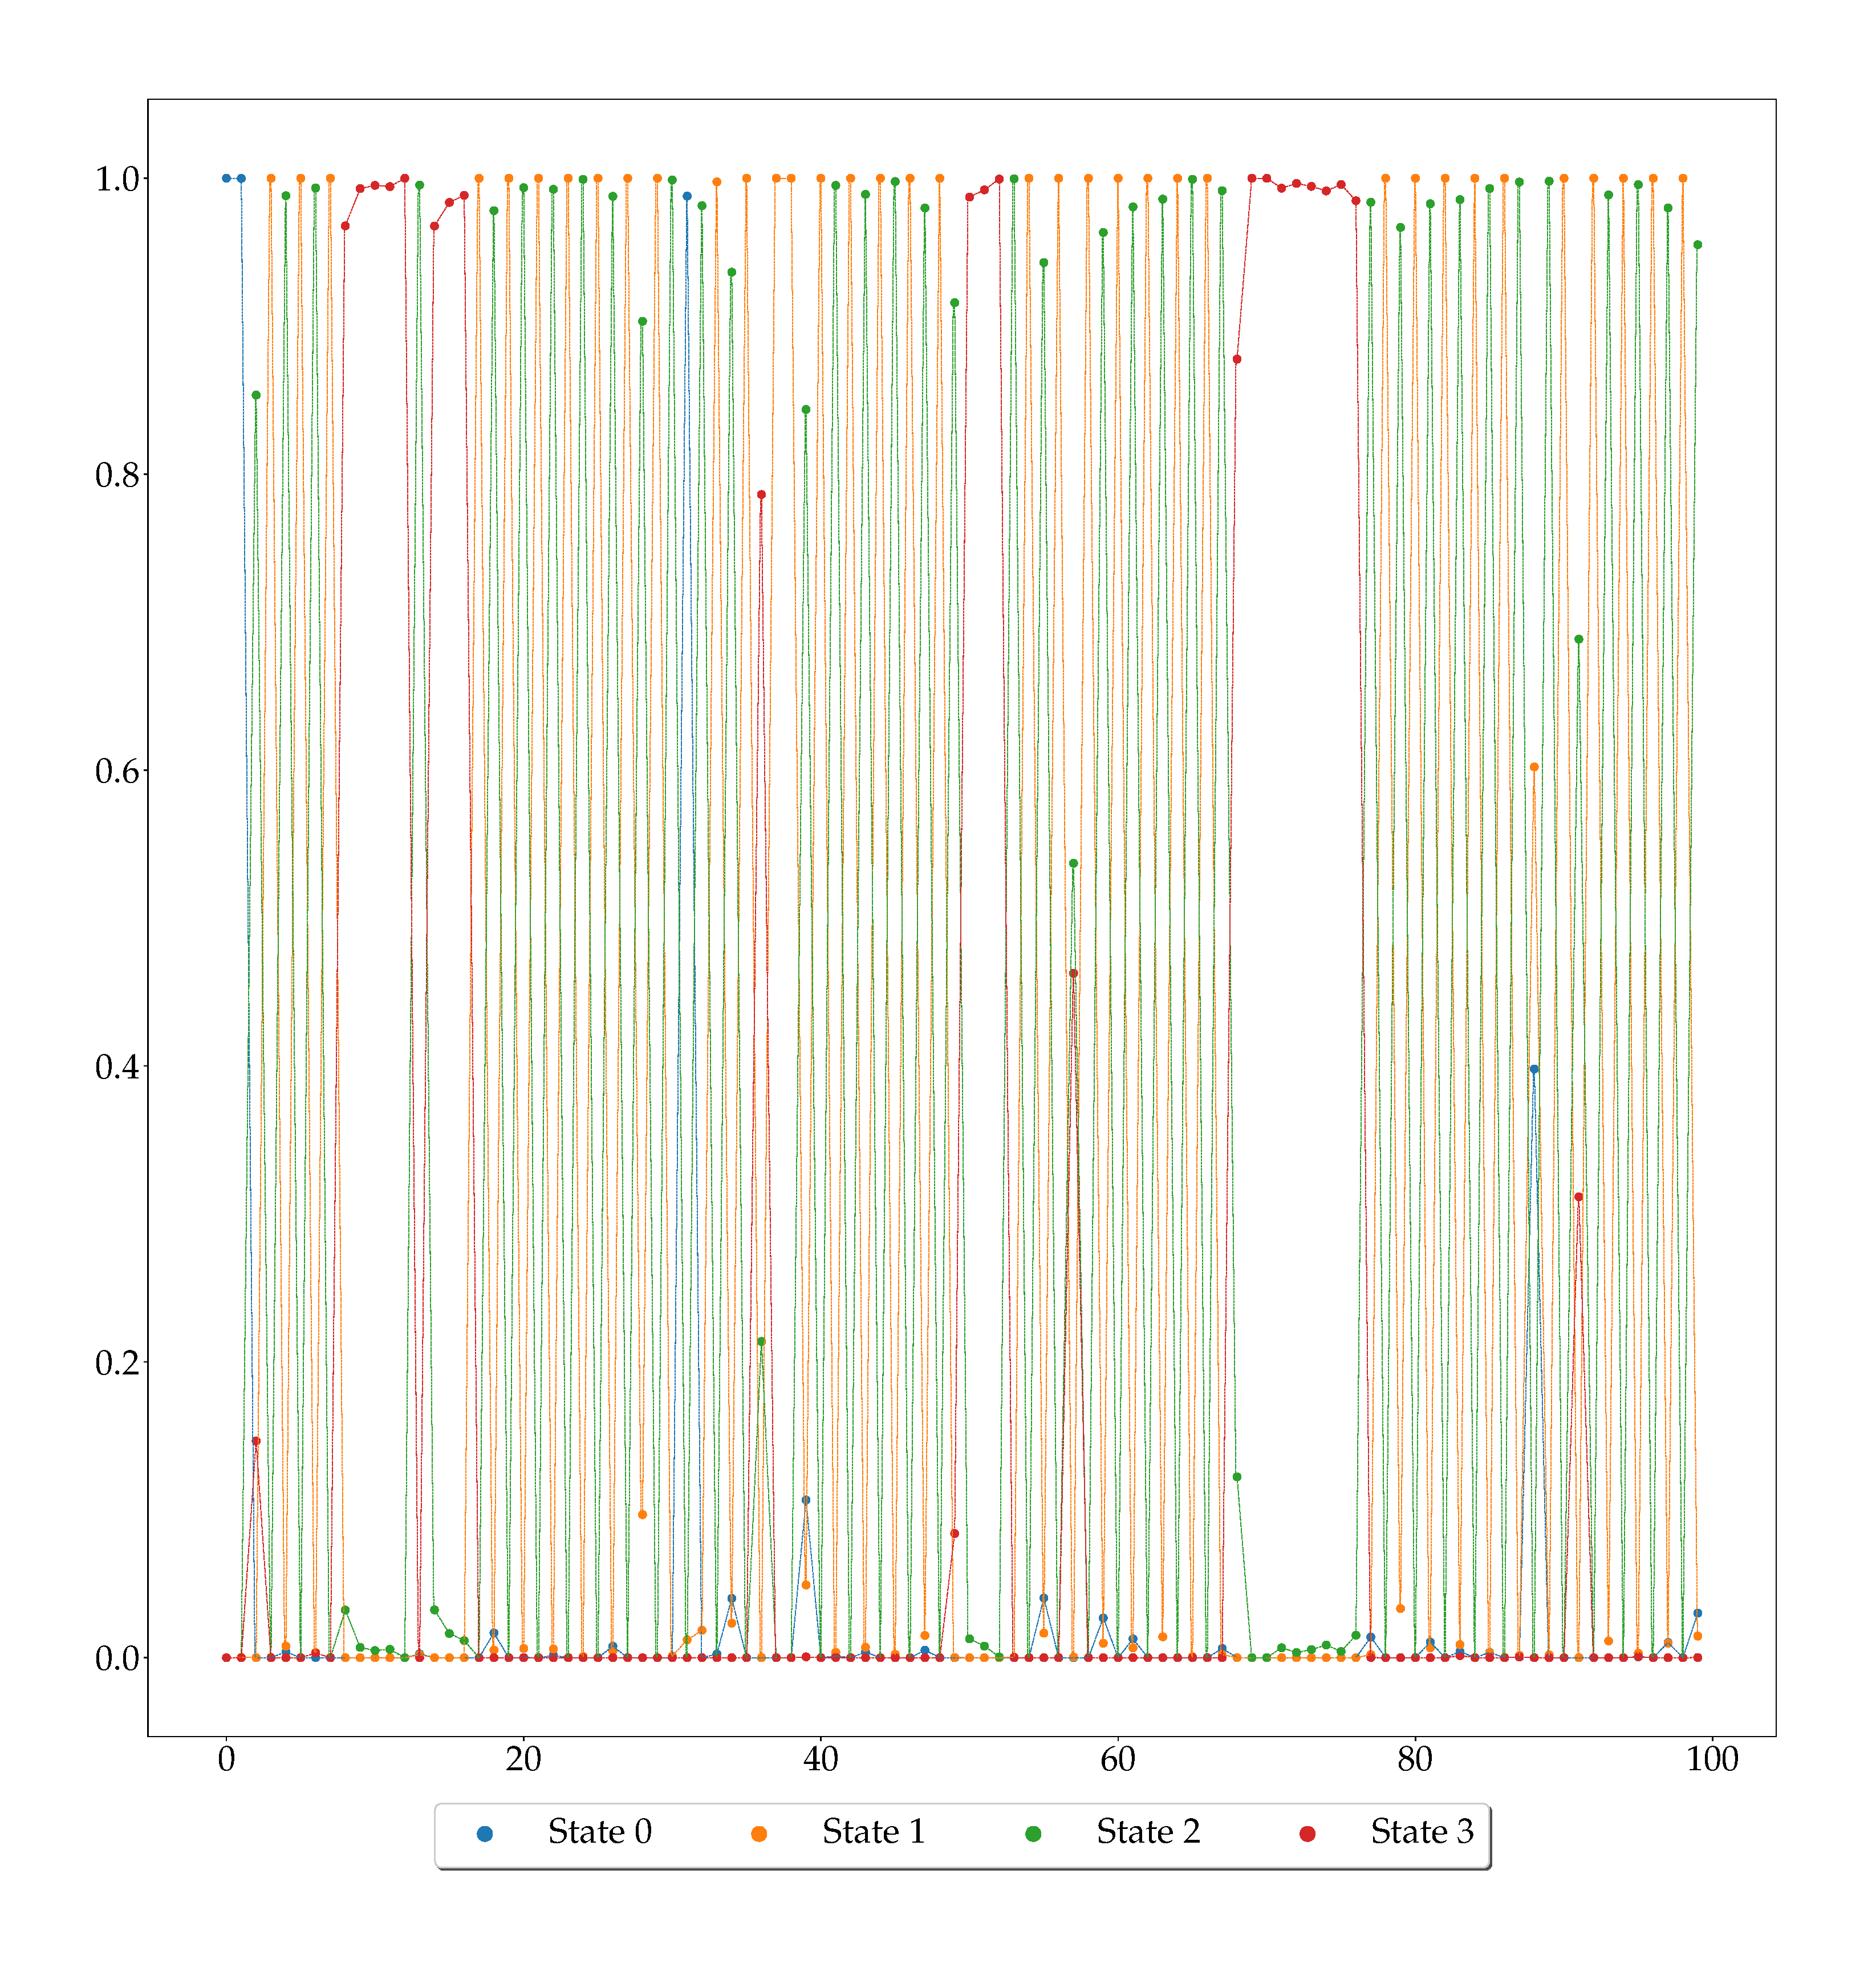
\includegraphics[width = 1.0\textwidth]{2_smoothing.eps}
	\caption{Filtering result for the first 100 datapoints}
	\label{fig_2_filtering}
\end{figure}


\subsection{}

En notant \(\bm{\theta} = \left(\pi, A, \bm{\mu}, \bm{\Sigma}\right)\) où \(\bm{\mu} = \{\mu_k\}_{k \in [\![1;4]\!]}\) et \(\bm{\Sigma} = \{\Sigma_k\}_{k \in [\![1;4]\!]}\), on exprime la log-vraisemblance incomplète de la manière suivante :
\begin{equation}
	\begin{split}
		\ell(\bm{\theta} ; \bm{u}) &= \ln \sum_{\bm{q}}p\left(\bm{q}, \bm{u} \mid \bm{\theta}\right)\\
		&= \ln \sum_{\bm{q}}r(\bm{q} \mid \bm{u}) \frac{p\left(\bm{q}, \bm{u} \mid \bm{\theta}\right)}{r(\bm{q} \mid \bm{u})} \quad \text{pour r quelconque}\\
		&\ge \sum_{\bm{q}}r(\bm{q} \mid \bm{u}) \ln \frac{p\left(\bm{q}, \bm{u} \mid \bm{\theta}\right)}{r(\bm{q} \mid \bm{u})} \quad \text{par l'inégalité de Jensen}\\
		&\ge \mathbb{E}_{r}[\ell_c(\bm{\theta} ; \bm{q}, \bm{u})]- H(r(\bm{q} \mid \bm{u})) = \mathcal{L}(r, \bm{\theta}, \bm{u})\\
	\end{split}
\end{equation}


avec \(\ell_c(\bm{\theta} ; \bm{q}, \bm{u})\), log-vraisemblance complète, dont l'expression est la suivante :
\begin{equation}
	\begin{split}

	\end{split}
\end{equation}

On a donc une borne inférieure de la log-vraisemblance incomplète, \(\mathcal{L}(r, \bm{\theta}, \bm{u})\). L'algorithme EM consiste en une montée alternée de cette borne inférieure par rapport à \(r\) et \(\bm{\theta}\). En choisissant \(r(\bm{q} \mid \bm{u}) = p(\bm{q} \mid \bm{u}, \bm{\theta})\), on maximise celle-ci, de sorte que les deux étapes de l'algorithme se résument de la manière suivante :
\begin{equation}
	\begin{split}
		E-step \quad r^{(s+1)} &= \operatorname{arg}\max_{r} \mathcal{L}(r, \bm{\theta}^{(s)}, \bm{u}) = p(\bm{q} \mid \bm{u}, \bm{\theta}^{(s)})\\
		M-step \quad \bm{\theta}^{(s+1)} &= \operatorname{arg}\max_{\bm{\theta}} \mathcal{L}(r^{(s+1)}, \bm{\theta}, \bm{u}) = \operatorname{arg}\max_{\bm{\theta}} \mathbb{E}_{r^{(s+1)}}(\ell_c(\bm{\theta} ; \bm{q}, \bm{u}))\\
	\end{split}
\end{equation}
où \(s\) dénote le nombre d'itérations de l'algorithme.



\section{}

\subsection{}

\begin{equation}
	\begin{split}
		X \indep Y \mid Z &\Leftrightarrow p(x, y \mid z) = p(x \mid z) p(y \mid z) \qquad \forall x, y, z \quad  \text{t.q.} \quad p(z) > 0 \\
		&\Leftrightarrow p(x, y, z) = p(x \mid z) p(y \mid z) p(z)\qquad \forall x, y, z \quad  \text{t.q.} \quad p(z) > 0 \\
		&\Leftrightarrow \frac{p(x, y ,z)}{p(y , z)} = p(x \mid z) \frac{p(y \mid z) p(z)}{p(y, z)} \qquad \forall x, y, z \quad  \text{t.q.} \quad p(y, z) > 0 \\
		&\Leftrightarrow p(x \mid y, z) = p(x \mid z) \qquad \forall x, y, z \quad  \text{t.q.} \quad p(y, z) > 0 \\
	\end{split}
\end{equation}

\subsection{}

Etant donné le modèle graphique orienté \(G\) :

\begin{equation}
	\begin{split}
		p \in \mathcal{L}(G) &\Leftrightarrow \forall x, y, z, t \quad p(x, y, z, t) = p(x)p(y)p(z \mid  x, y) p(t \mid z)
	\end{split}
\end{equation}



\subsection{}

\textit{Non traité}.

\section{Distributions factorisant sur un graphe}

\subsection{}
\textit{Non traité}.

\subsection{}
\textit{Non traité}.

\clearpage

\section{Entropie et information mutuelle}

\subsection{Entropie}

\subsubsection{}

Avec les conventions définies :

\begin{equation}
	\begin{split}
		p_X(x) &= \mathbb{P}(X = x) < 1 \Rightarrow p_X(x)\log(p_X(x)) < 0 \Rightarrow -\sum_{x \in \mathcal{X}} p_X(x)\log(p_X(x)) = H(X) \geq 0 \\
		H(X) &= 0 \Rightarrow \forall x \in \mathcal{X},\, p_X(x)\log(p_X(x)) = 0 \Rightarrow \forall x \in \mathcal{X},\, p_X(x) = 1 \Rightarrow \text{X is constant with probability 1}
	\end{split}
	\label{eq_31a}
\end{equation}

\subsubsection{}

Par définition de la Kullback-Leibler divergence il vient :

\begin{equation}
	\begin{split}
		D(p_X \parallel q) &= \sum_{x \in \mathcal{X}}p_X(x)\log\frac{p_X(x)}{q(x)}\\
		&= -\sum_{x \in \mathcal{X}}p_X(x)\log q(x) - H(X) \\
		&= -\sum_{x \in \mathcal{X}}p_X(x)\log\frac{1}{|X|} - H(X) \quad \text{puisque} \quad \forall x \in \mathcal{X},\, q(x) = \frac{1}{k} = \frac{1}{k}\\
		&= \log k\sum_{x \in \mathcal{X}}p_X(x) - H(X)\\
		&= \log k - H(X) \quad \text{car} \quad \sum_{x \in \mathcal{X}}p_X(x) = 1
	\end{split}
	\label{eq_31b}
\end{equation}

\subsubsection{}
Avec les équations~\eqref{eq_31a} et \eqref{eq_31b}, on a directement

\begin{equation}
	\log k - H(X) = D(p_X \parallel q) \leq \log k
\end{equation}

\subsection{Information mutuelle}

\subsubsection{}
Par définition de l'information mutuelle :

\begin{equation}
	\begin{split}
		I(X_1, X_2) &= \sum_{(x_1,x_2)\in\mathcal{X}_1\times\mathcal{X}_2} p_{1, 2}(x_1,x_2) \log \frac{p_{1, 2}(x_1,x_2)}{p_1(x_1)\,p_2(x_2)}\\
		I(X_1, X_2) &= D(p_{1, 2} \parallel p_1p_2) \quad \text{par définition de la Kullback-Leibler divergence}
	\end{split}
\end{equation}

Or la Kullback-Leibler divergence est positive pour toute paire \((p_{1, 2}, p_1p_2)\) de distributions, donc \(I(X_1, X_2) \geq 0\).

\subsubsection{}

Toujours avec la défintion de l'information mutuelle :

\begin{equation}
	\begin{split}
		I(X_1, X_2) &= \sum_{(x_1,x_2)\in\mathcal{X}_1\times\mathcal{X}_2} p_{1, 2}(x_1,x_2) \log \frac{p_{1, 2}(x_1,x_2)}{p_1(x_1)\,p_2(x_2)}\\
		I(X_1, X_2) &= \sum_{(x_1,x_2)\in\mathcal{X}_1\times\mathcal{X}_2} p_{1, 2}(x_1,x_2) \log p_{1, 2}(x_1,x_2)\\ &- \sum_{(x_1,x_2)\in\mathcal{X}_1\times\mathcal{X}_2} p_{1, 2}(x_1,x_2) \log \left(p_1(x_1)p_2(x_2)\right)\\
		I(X_1, X_2) &= -H(X_1, X_2)\\
		&- \sum_{x_1 \in\mathcal{X}_1} \left(\sum_{x_2 \in\mathcal{X}_2}p_{1, 2}(x_1,x_2)\right) \log \left(p_1(x_1)\right)\\
		&- \sum_{x_2 \in\mathcal{X}_2} \left(\sum_{x_1 \in\mathcal{X}_1}p_{1, 2}(x_1,x_2)\right) \log \left(p_2(x_2)\right)\\
		I(X_1, X_2) &= -H(X_1, X_2)\\
		&- \sum_{x_1 \in\mathcal{X}_1} p_{1}(x_1) \log \left(p_1(x_1)\right)\\
		&- \sum_{x_2 \in\mathcal{X}_2} p_{2}(x_2) \log \left(p_2(x_2)\right)\\
		I(X_1, X_2) &= H(X_1) + H(X_2) - H(X_1, X_2)
	\end{split}
	\label{eq_32b}
\end{equation}

Et ainsi l'information mutuelle peut s'écrire uniquement à partir des entropies de \(X_1\), \(X_2\) et de \((X_1, X_2)\).

\subsubsection{}

D'après l'éqiation~\eqref{eq_32b}, on peut réecrire :

\begin{equation}
	\begin{split}
		H(X_1, X_2) - \left(H(X_1) + H(X_2)\right) &=  - I(X_1, X_2)\\
		H(X_1, X_2) - \left(H(X_1) + H(X_2)\right) &\leq 0 \quad \text{puisque},\, I(X_1, X_2) \geq 0
	\end{split}
	\label{eq_32c}
\end{equation}

D'après l'équation~\eqref{eq_32c}, pour \(p_1\) et \(p_2\) données, l'entropie maximale correspond à \(I(X_1, X_2) = 0\), c'est-à-dire \(D(p_{1, 2} \parallel p_1p_2) = 0\) d'après l'équation~\eqref{eq_31b}. Or la Kullback-Leibler divergence s'anulle si et seulement si les distributions sont identiques. On a alors \(p_{1,2} = p_1p_2\), ce qui correspond à \(X_1 \indep X_2\).

\section{Gaussian Mixtures}

\subsection{K-means}
\end{document}
